\section{Appendix}

\subsection{Community labels of super-vertices}

We also attempt two different variations of Parallel Leiden algorithm, one where the community labels of super-vertices (upon aggregation) is based on the local-moving phase (\textit{move-based}), and the other where the community labels of super-vertices is based on the refinement phase (\textit{refine-based}). Our observations indicate that both approaches have roughly the same runtime and modularity on average, as indicated by Figures \ref{fig:leidenreopt-runtime} and \ref{fig:leidenreopt-modularity}. Accordingly, we stick to the move-based approach, which is the one recommended by Traag et al. \cite{com-traag19}. However, refine-based approach may be more suitable for the design of dynamic Leiden algorithm (for dynamic graphs).

\begin{figure}[hbtp]
  \centering
  \subfigure{
    \label{fig:leidenreopt-runtime--all}
    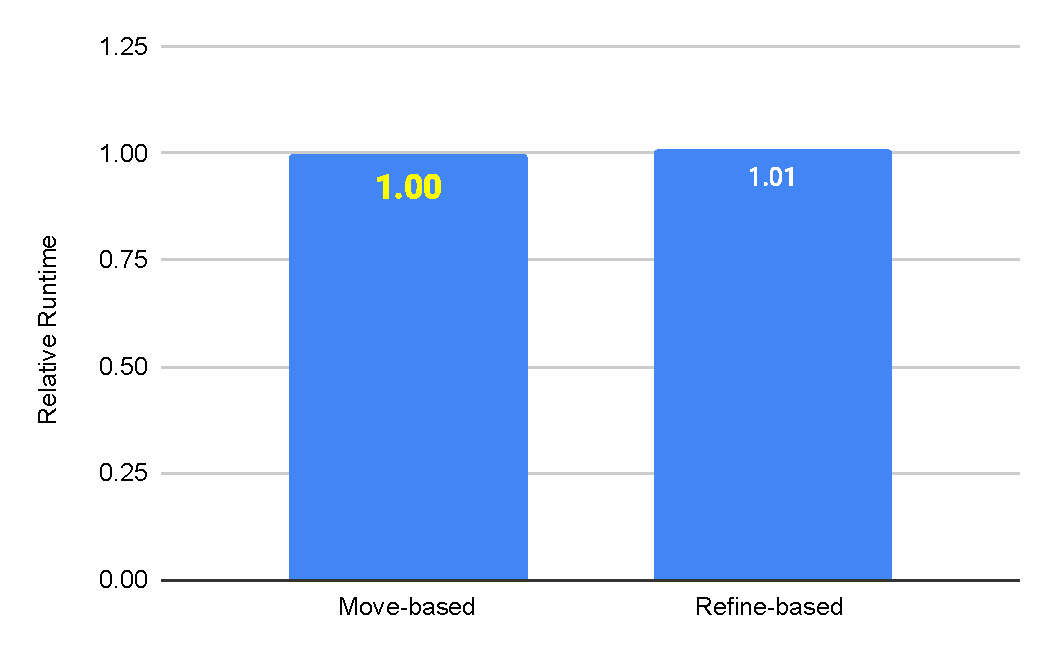
\includegraphics[width=0.98\linewidth]{out/leidenreopt-runtime.pdf}
  } \\[-2ex]
  \caption{Average relative runtime for \textit{move-based} and \textit{refine-based} communities for super-vertices upon aggregation with parallel Leiden algorithm, for all graphs in the dataset.}
  \label{fig:leidenreopt-runtime}
\end{figure}

\begin{figure}[hbtp]
  \centering
  \subfigure{
    \label{fig:leidenreopt-modularity--all}
    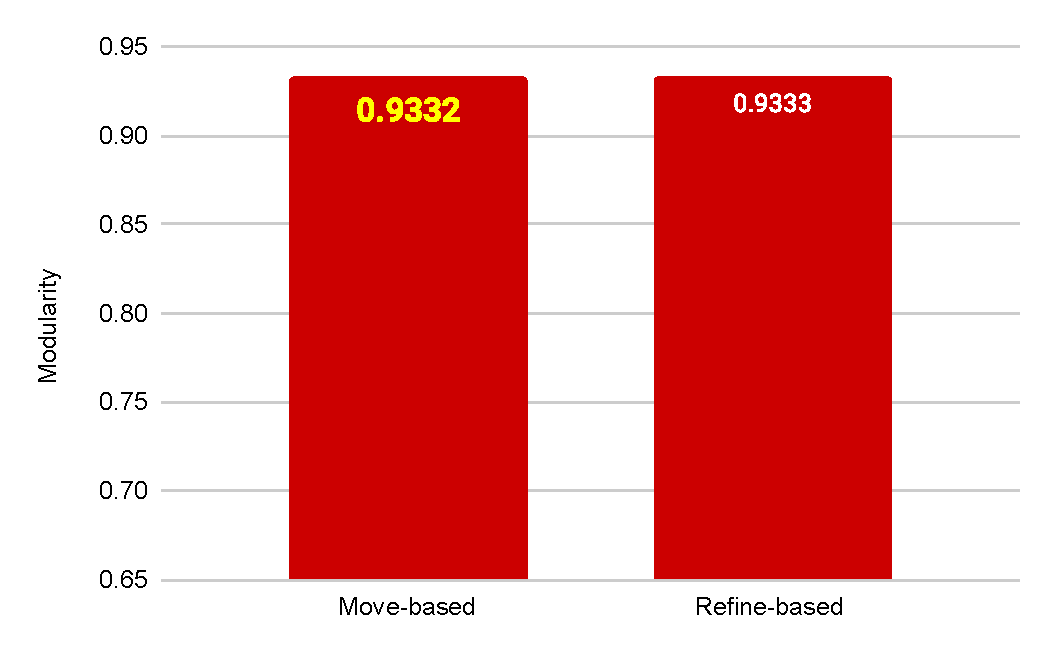
\includegraphics[width=0.98\linewidth]{out/leidenreopt-modularity.pdf}
  } \\[-2ex]
  \caption{Average modularity for \textit{move-based} and \textit{refine-based} communities for super-vertices upon aggregation with parallel Leiden algorithm, for all graphs in the dataset.}
  \label{fig:leidenreopt-modularity}
\end{figure}





\subsection{Finding disconnected communities}

We now outline our parallel algorithm for identifying disconnected communities, given the original graph and the community membership of each vertex. The core concept involves determining the size of each community, selecting a vertex from each community, traversing within the community from that vertex (avoiding adjacent communities), and marking a community as disconnected if all its vertices cannot be reached. We explore four distinct approaches, differing in the use of parallel Depth-First Search (DFS) or Breadth-First Search (BFS) and whether per-thread or shared \textit{visited} flags are employed. If shared visited flags are used, each thread scans all vertices but processes only its assigned community based on the community ID. Our findings suggest that utilizing parallel BFS traversal with a shared flag vector yields the fastest results. As this is not a heuristic algorithm, all approaches produce identical outcomes. Algorithm \ref{alg:disconnected} illustrates the pseudocode for this approach. Here, the \texttt{disconnectedCommunities()} function takes the input graph $G$ and the community membership $C$ as input, and it returns the disconnected flag $D$ for each community.

\begin{algorithm}[hbtp]
\caption{Finding disconnected communities in parallel.}
\label{alg:disconnected}
\begin{algorithmic}[1]
\Require{$G$: Input graph}
\Require{$C$: Community membership of each vertex}
\Ensure{$D$: Disconnected flag for each community}
\Ensure{$S$: Size of each community}
\Ensure{$f_{if}$: Perform BFS to vertex $j$ if condition satisfied}
\Ensure{$f_{do}$: Perform operation after each vertex is visited}
\Ensure{$reached$: Number of vertices reachable from $i$ to $i$'s community}
\Ensure{$work_t$: Work-list of current thread}

\Statex

\Function{disconnectedCommunities}{$G, C$} \label{alg:disconnected--begin}
  \State $D \gets \{\}$ \textbf{;} $vis \gets \{\}$ \label{alg:disconnected--init}
  \State $S \gets communitySizes(G, C)$ \label{alg:disconnected--sizes}
  \ForAll{\textbf{threads in parallel}} \label{alg:disconnected--threads-begin}
    \ForAll{$i \in V$} \label{alg:disconnected--loop-begin}
      \State $c \gets C[i]$ \textbf{;} $reached \gets 0$ \label{alg:disconnected--unreached}
      \State $\rhd$ Skip if community $c$ is empty, or
      \State $\rhd$ does not belong to work-list of current thread.
      \If{$S[c] = 0$ \textbf{or} $c \notin work_t$} \textbf{continue} \label{alg:disconnected--work}
      \EndIf
      \State $f_{if} \gets (j) \implies C[j] = c$
      \State $f_{do} \gets (j) \implies reached \gets reached + 1$
      \State $bfsVisitForEach(vis, G, i, f_{if}, f_{do})$ \label{alg:disconnected--bfs}
      \If{$reached < S[c]$} $D[c] \gets 1$ \label{alg:disconnected--mark}
      \EndIf
      \State $S[c] \gets 0$ \label{alg:disconnected--processed}
    \EndFor \label{alg:disconnected--loop-end}
  \EndFor \label{alg:disconnected--threads-end}
  \Return{$D$}
\EndFunction \label{alg:disconnected--end}
\end{algorithmic}
\end{algorithm}


We now explain Algorithm \ref{alg:disconnected} in detail. First, in line \ref{alg:disconnected--init}, the disconnected community flag $D$, and the visited vertices flags $vis$ are initialized. In line \ref{alg:disconnected--sizes}, the size of each community $S$ is obtained in parallel using the \texttt{communitySizes()} function. Subsequently, each thread processes each vertex $i$ in the graph $G$ in parallel (lines \ref{alg:disconnected--loop-begin}-\ref{alg:disconnected--loop-end}). In line \ref{alg:disconnected--unreached}, the community membership of $i$ ($c$) is determined, and the count of vertices reached from $i$ is initialized to $0$. If community $c$ is empty or not in the work-list of the current thread $work_t$, the thread proceeds to the next iteration (line \ref{alg:disconnected--work}). If however the community $c$ is non-empty and in the work-list of the current thread $work_t$, BFS is performed from vertex $i$ to explore vertices in the same community, using lambda functions $f_{if}$ to conditionally perform BFS to vertex $j$ if it belongs to the same community, and $f_{do}$ to update the count of $reached$ vertices after each vertex is visited during BFS (line \ref{alg:disconnected--bfs}). If the number of vertices $reached$ during BFS is less than the community size $S[c]$, the community $c$ is marked as disconnected (line \ref{alg:disconnected--mark}). Finally, the size of the community $S[c]$ is updated to $0$, indicating that the community has been processed (line \ref{alg:disconnected--processed}). Note that the work-list $work_t$ for each thread with ID $t$, is defined as a set containing communities $[t\chi,\ t(\chi+1))\ \cup\ [T\chi + t\chi,\ T\chi + t(\chi+1))\ \cup\ \ldots$, where $\chi$ is the chunk size, and $T$ is the number of threads. We use a chunk size of $\chi = 1024$.




\subsection{Indirect Comparison with State-of-the-art Leiden Implementations}
\label{sec:comparison-indirect}

Finally, we conduct an indirect comparison of the performance of our multicore implementation of the Leiden algorithm with other similar state-of-the-art implementations, as listed in Table \ref{tab:compare}. Hu et al. \cite{huparleiden} introduce ParLeiden, a parallel Leiden implementation for distributed environments, which uses thread locks and efficient buffers, to resolve community joining conflicts and reduce communication overheads. They refer to their single node version of ParLeiden as ParLeiden-S, and their distributed version as ParLeiden-D. On a cluster with $8$ nodes, with each node being equipped with a $48$ core CPU, Hu et al. observe a speedup of $12.3\times$, $9.9\times$, and $1.32\times$ for ParLeiden-S, ParLeiden-D, and a baseline Leiden implemented on KatanaGraph, on the \textit{com-LiveJournal} graph, with respect to original Leiden \cite{com-traag19} (refer to Table 2 in their paper \cite{huparleiden}). In contrast, on the same graph, we observe a speedup of $219\times$ relative to original Leiden. Consequently, our Leiden implementation outperforms ParLeiden-S, ParLeiden-D, and KatanaGraph Leiden by approximately $18\times$, $22\times$, and $166\times$ respectively\ignore{ (all achieved without GPU)}.
